\section{Electricity \& Magnetism}

This section covers material related to the E\&M portion of the exam.
Most of these subsections go into more depth than is required for the PGRE.
Gauss's law, Faraday's law, and radiation originating from charged particles are consistently tested on the practice exams.
Method of images is also something to brush up on.

\subsection{Electrostatics}

\subsubsection{Coulomb's Law}
Force Law: \(\displaystyle\mathbf{F}_E=k_e\frac{q_1q_2}{\scriptr^2}\hat{\scriptr}\)\\\\*
Electric Field:\\*
\(\displaystyle\mathbf{F}_E=q\mathbf{E}\)\\*
\(\displaystyle\mathbf{E}=k_e\sum_i\frac{q_i}{\scriptr_i^2}\hat{\scriptr}_i\to k_e\int\frac{\hat{\scriptr}}{\scriptr^2}\mathrm{d}q\)\\\\*
Electric Field Example: E-field along \(z\)-axis due to a ring of charge \(Q\) centered at the origin and in the \(x\)-\(y\) plane: \(\displaystyle\mathbf{E}=\frac{k_eQd}{(R^2+z^2)^{3/2}}\hat{z}\)

\subsubsection{Gauss's Law}
Electric Flux: \(\Phi_E=\int_S\mathbf{E}\cdot\,\mathrm{d}\mathbf{a}\)\\*
Through a Closed Surface: \(\displaystyle\Phi_E=\oint_{\delta V}\mathbf{E}\cdot\,\mathrm{d}\mathbf{a}\)\\*
Differential Form: \(\nabla\cdot\mathbf{E}=\displaystyle\frac{\rho}{\epsilon_0}\)\\*
Integral Form: \(\displaystyle\oint_{\delta V}\mathbf{E}\cdot\,\mathrm{d}\mathbf{a}=\frac{Q_{enc}}{\epsilon_0}\)\\\\*
Common Uses of Gauss's Law:
\begin{itemize}
\item Spherical Symmetry: Inside uniformly charged sphere of radius \(a \to\) \(\displaystyle E=\frac{k_eQ}{a^3}r=\frac{\rho}{3\epsilon_0}r\)
\item Cylindrical Symmetry: Outside cylinder of radius \(b\) with uniform surface charge \(\to\) \(\displaystyle E=\frac{\sigma b}{\epsilon_0}\frac{1}{r}\)
\item Planar Surface: Near plate with uniform surface charge \(\to\) \(\displaystyle E=\frac{\sigma}{2\epsilon_0}\)
\end{itemize}
Gauss's law is also useful in showing that all the net charge on a conductor must reside on its surface, as well as that there is no E-field inside a conductor and, therefore, no net force on a particle placed in a conductor.\\*
Gauss's law is typically the easiest way to calculate E-fields when enough spatial symmetry is present.

\newpage
\subsubsection{Electric Potential}
\(\nabla\times\mathbf{E}=\vec{0}\to\mathbf{E}=-\nabla V \to -\nabla^2 V=\displaystyle\frac{\rho}{\epsilon_0}\)\\\\*
Electric Potential: \(\displaystyle V(\mathbf{b})-V(\mathbf{a})= -\int_\mathbf{a}^\mathbf{b}\mathbf{E}\cdot\,\mathrm{d}\mathbf{s}\)\\\\*
If \(\mathbf{a}\) is taken to be a reference where \(V(\mathbf{a})=0\), then \(\displaystyle V(\mathbf{r})= -\int_\mathbf{O}^\mathbf{r}\mathbf{E}\cdot\,\mathrm{d}\mathbf{s}\)\\\\*
\(\displaystyle V=k_e\sum_i\frac{q_i}{\scriptr_i} \to k_e\int\frac{\mathrm{d}q}{\scriptr}\)\\*
A conductor is an equipotential and the \(\mathbf{E}\) field is \(\bot\) to the surface just above a conductor (else the surface charge would move).\\*
Electric Potential Example: Potential along \(z\)-axis due to a ring of charge \(Q\) centered at the origin and in the \(x\)-\(y\) plane \(\to\) \(\displaystyle\ V=\frac{k_eQ}{\sqrt{R^2+z^2}}\)

\subsubsection{Electrostatic Force on a Conductor}
Force per unit area: \(\mathbf{f}=\sigma\mathbf{E}_{ave}=\frac{1}{2}\sigma(\mathbf{E}_{above}-\mathbf{E}_{below})\)\\*
(This actually applies to any surface charge.)\\\\*
For a conductor: \(\mathbf{f}=\frac{1}{2\epsilon_0}\sigma^2\hat{\mathbf{n}}\)

\subsubsection{Electric Dipole}
Electric Dipole Moment: \(\mathbf{p}=q\mathbf{d}\) where \(\mathbf{d}\) is the displacement vector pointing from the negative charge (\(-q\)) to the positive charge (\(q\))\\*
\(\displaystyle\mathbf{p}=\int{\mathbf{r'}\rho(\mathbf{r}')\mathrm{d}v'}\)\\\\*
The electric potential from a dipole:\\*
\(\displaystyle V(\mathbf{r})=\frac{1}{4\pi\epsilon_0}=\frac{\mathbf{p}\cdot\hat{\mathbf{r}}}{r^2}\)\\\\*
The field from a dipole:\\*
\(\displaystyle E_{dipole}\propto \frac{p}{r^3}\)\\*
Specifically, \(\displaystyle \mathbf{E}_{dipole}=\frac{1}{4\pi\epsilon_0}\frac{1}{r^3}\left[3\left(\mathbf{p}\cdot\hat{\mathbf{r}}\right)\hat{\mathbf{r}}-\mathbf{p}\right]\)\\\\*
Effect of an external \(\mathbf{E}\) field on a dipole:\\*
Force: \(\mathbf{F}=\left(\mathbf{p}\cdot\nabla\right)\mathbf{E}\)\\*
Torque: \(\vec{\tau}=\mathbf{p}\times\mathbf{E}\)\\*
Potential Energy: \(U=-\mathbf{p}\cdot\mathbf{E}\)

\subsubsection{Dielectrics}
The dipole moment per unit volume is called the polarization \(\mathbf{P}\).\\*
\(\mathbf{P}\cdot\hat{\mathbf{n}}=\sigma_{bound}\)\\*
\(-\nabla\cdot\mathbf{P}=\rho_{bound}\)\\\\*
\(\displaystyle V(\mathbf{r})=\frac{1}{4\pi\epsilon_0}\int{\frac{\hat{\mathbf{\scriptr}}\cdot\mathbf{P}(\mathbf{r}')}{\scriptr^2}\mathrm{d}v'}\)\\\\*
The electric displacement is \(\mathbf{D}=\epsilon_0\mathbf{E}+\mathbf{P}\).\\*
\(\nabla\cdot\mathbf{D}=\rho_{free}\to \displaystyle\oint_{\delta V}\mathbf{D}\cdot\,\mathrm{d}\mathbf{a}=Q_{free_{enc}}\)\\\\*

Linear Dielectrics:\\*
Dielectric Constant: \(\displaystyle\kappa=\frac{\epsilon}{\epsilon_0}\) (note: \(\kappa\geq 1\) typically)\\*
\(\mathbf{P}=(\epsilon-\epsilon_0)\mathbf{E}\)\\*
\(\mathbf{D}=\epsilon\mathbf{E}=\kappa\epsilon_0\mathbf{E}\)\\\\*
A convenient way to calculate \(\displaystyle\sigma_{bound}\) is to use \(\mathbf{D}=\epsilon\mathbf{E}\) with \(\displaystyle\oint_{\delta V}\mathbf{D}\cdot\,\mathrm{d}\mathbf{a}=Q_{free_{enc}}\) to get \(\mathbf{P}\) and finally use the relation \(\mathbf{P}\cdot\hat{\mathbf{n}}=\sigma_{bound}\).

\subsubsection{Energy in an Electrostatic Field}
\(\displaystyle U=\frac{k_e}{2}\sum_j\sum_{i\neq j}\frac{q_iq_j}{r_{ij}} \)\\*
\(\displaystyle U=\frac{\epsilon_0}{2}\int{E^2\mathrm{d}v}\)\\*
\(\displaystyle U=\frac{1}{2}\int{\mathbf{D}\cdot\mathbf{E}\hspace{2pt}\mathrm{d}v}\)

\subsubsection{Method of Images}
Force behaves as if there was an actual image charge present.\\*
Energy, however, needs to be calculated using only regions ``outside'' the conductor. (\(\mathbf{E}=\mathbf{0}\) ``inside'')\\*
For planar conductor, replace the conductor with a mirror image of the charge distribution with opposite charge.\\*
For spherical conductor of radius \(R\), replace the conductor with a charge \(q'\) a distance \(b\) from the origin.
(\(r\) is the distance \(q\) is from the center of the sphere)
\begin{eqnarray}
\displaystyle q'&=&\frac{-R}{r}q \nonumber \\
\displaystyle b&=&\frac{R^2}{r} \nonumber
\end{eqnarray}

\subsubsection{Separation of Variables}
Used to solve Laplace's equation: \(\nabla^2 V(\mathbf{r})=0\)\\\\*
Decompose \(V(\mathbf{r})\) into separate, independent functions of the coordinates.\\\\*
Use boundary conditions to find relationship between the series coefficients and exploit the orthogonality (or orthonormality) of the trigonometric functions, \(P_l\), or \(Y_l^m\).\\\\*
For Cartesian coordinates you must set up and solve each scenario from scratch.\\*
In spherical polar coordinates with azimuthal symmetry, use:\\*
\(\displaystyle V(r,\theta)=\sum_{l=0}^\infty\left(A_lr^l+\frac{B_l}{r^{l+1}}\right)P_l(\cos{\theta})\)

\subsection{Magnetostatics}

\subsubsection{Current}
\(\displaystyle I=\frac{\mathrm{d}q}{\mathrm{d}t}\)\\\\*
Drift Velocity of Charge Carriers: \(I=nqv_DA\)\\*
Current Density: \(J=\frac{I}{A}=nqv_D\to \mathbf{J}=nq\mathbf{v}_D\)\\\\*
Linear Current: \(\mathbf{I}=\lambda \mathbf{v}\)\\*
Surface Current: \(\mathbf{K}=\sigma \mathbf{v}\)\\*
Volume Current: \(\mathbf{J}=\rho \mathbf{v}\)

\subsubsection{Biot-Savart's Law}
\(\displaystyle\mathbf{B}=\frac{\mu_0}{4\pi}\int\frac{\mathbf{I}\times\hat{\scriptr}}{\scriptr^2}\mathrm{d}s'\)\\\\*
\(\displaystyle\mathbf{B}=\frac{\mu_0}{4\pi}\int\frac{\mathbf{K}\times\hat{\scriptr}}{\scriptr^2}\mathrm{d}a'\)\\\\*
\(\displaystyle\mathbf{B}=\frac{\mu_0}{4\pi}\int\frac{\mathbf{J}\times\hat{\scriptr}}{\scriptr^2}\mathrm{d}v'\)\\\\*
Common Uses of Biot-Savart's Law:
\begin{itemize}
\item Circular wire arc at center of curvature: \(\displaystyle B=\frac{\mu_0I\theta}{4\pi R}\)
\item Circular current loop along axis: \(\displaystyle B=\frac{\mu_0I}{2}\frac{r^2}{\left(R^2+z^2\right)^{3/2}}\)
\end{itemize}
Both of these give \(\displaystyle B=\frac{\mu_0I}{2R}\) at the center of a current loop.
Far away from the loop (along the axis) the B-field behaves like \(\displaystyle B\propto\frac{1}{z^3}\).

\subsubsection{Amp\`ere's Law}
DifferentialForm: \(\nabla\times\mathbf{B}=\mu_0\mathbf{J}\)\\*
Integral Form: \(\displaystyle\oint_{\delta S}\mathbf{B}\cdot\,\mathrm{d}\mathbf{l}=\mu_0 I_{enc}\)\\\\*
Common Uses of Amp\`ere's Law:
\begin{itemize}
\item Long wire: \(\displaystyle B=\frac{\mu_0I}{2\pi r}\)
\item Solenoid/Toroid: \(\displaystyle B=\mu_0 n I\) where \(\displaystyle n=\frac{N_{turns}}{l}\) for a solenoid and \(\displaystyle\frac{N_{turns}}{2\pi R}\) for a toroid
\end{itemize}

\subsubsection{Magnetic Forces on Objects}
Particle: \(\mathbf{F}_B=q\mathbf{v}\times\mathbf{B}\)\\*
Wire:  \(\mathbf{F}_B=I\mathbf{L}\times\mathbf{B}\) (\(\mathbf{L}\) connects \emph{endpoints} of wire)\\*
The net magnetic force acting on any closed current loop in \emph{uniform} magnetic field is zero (\(\mathbf{L}=\mathbf{0}\)), but the torque isn't necessarily zero.\\*
\(\vec{\tau}=I\mathbf{A}\times\mathbf{B}\) where \(\mathbf{A}\) is the area enclosed by the loop\\\\*
\(\mathbf{F}=\int I(\mathrm{d}\mathbf{s}\times\mathbf{B})\)\\*
\(\mathbf{F}=\int (\mathbf{K}\times\mathbf{B})\mathrm{d}a\)\\*
\(\mathbf{F}=\int (\mathbf{J}\times\mathbf{B})\mathrm{d}v\)\\\\*
Cyclotron (angular) frequency:
\begin{eqnarray}
ma&=&qvB \nonumber\\
m\omega^2R&=&q\omega RB \nonumber\\
\omega_{cyclotron}&=&\frac{qB}{m} \nonumber
\end{eqnarray}
Force per length between two current carrying wires separated by a distance \(a\): \(\displaystyle\frac{F_B}{l}=\frac{\mu_0I_1I_2}{2\pi a}\) (currents in the same direction attract while opposite currents repel)

\subsubsection{Magnetic Flux}
\(\Phi_B=\int_S\mathbf{B}\cdot\,\mathrm{d}\mathbf{a}\)\\\\*
\(\displaystyle\Phi_B=\oint_{\delta V}\mathbf{B}\cdot\,\mathrm{d}\mathbf{a}=0\to\nabla\cdot\mathbf{B}=\mathbf{0}\)\\*
This last statement just means there are no magnetic monopoles, or ``magnetic charges.''

\subsubsection{Magnetic Vector Pontential}
\(\nabla\cdot\mathbf{B}=\mathbf{0}\to\mathbf{B}=\nabla\times\mathbf{A}\)\\*
\(\nabla^2\mathbf{A}=-\mu_0\mathbf{J}\)\\\\*
\(\displaystyle\mathbf{A}=\frac{\mu_0}{4\pi}\int\frac{I}{\scriptr}\mathrm{d}\mathbf{s}'\)\\\\*
\(\displaystyle\mathbf{A}=\frac{\mu_0}{4\pi}\int\frac{\mathbf{K}(\mathbf{r}')}{\scriptr}\mathrm{d}a'\)\\\\*
\(\displaystyle\mathbf{A}=\frac{\mu_0}{4\pi}\int\frac{\mathbf{J}(\mathbf{r}')}{\scriptr}\mathrm{d}v'\)

\subsubsection{Magnetic Dipole}
\(\mathbf{m} =\int I\mathrm{d}\mathbf{a}\)\\\\*
The magnetic vector potential from a dipole:\\*
\(\displaystyle\mathbf{A}_{dipole}=\frac{\mu_0}{4\pi}\frac{\mathbf{m}\times\hat{\mathbf{r}}}{r^2}\)\\\\*
The field from a dipole:\\*
\(\displaystyle \mathbf{B}_{dipole}=\frac{\mu_0}{4\pi}\frac{1}{r^3}\left[3\left(\mathbf{m}\cdot\hat{\mathbf{r}}\right)\hat{\mathbf{r}}-\mathbf{m}\right]\)\\\\*
Effect of an external \(\mathbf{B}\) field on a dipole:\\*
Force: \(\mathbf{F}=\nabla(\mathbf{m}\cdot\mathbf{B})\)\\*
Torque: \(\vec{\tau}=\mathbf{m}\times\mathbf{B}\)\\*
Potential Energy: \(U=-\mathbf{m}\cdot\mathbf{B}\)

\subsubsection{Dia-Para-Ferromagnetic Materials}
The magnetic dipole moment per unit volume is called the magnetization \(\mathbf{M}\).\\*
\(\nabla\times\mathbf{M}=\mathbf{J}_{bound}\)\\*
\(\mathbf{M}\times\hat{\mathbf{n}}=\mathbf{K}_{bound}\)\\\\*
\(\displaystyle\mathbf{A}(\mathbf{r})=\frac{\mu_0}{4\pi}\int\frac{\mathbf{M}\times\hat{\scriptr}}{\scriptr^2}\mathrm{d}v'\)\\\\*
\(\displaystyle\mathbf{H}=\frac{1}{\mu_0}\mathbf{B}-\mathbf{M}\)\\\\*
\(\nabla\times\mathbf{H}=\mathbf{J}_{free}\)\\*
\(\displaystyle\oint\mathbf{H}\cdot\mathrm{d}\mathbf{l}=I_{free_{enc}}\)\\\\*
For Linear Materials: \(\mathbf{H}=\mu\mathbf{B}\)
\begin{itemize}
\item Diamagnets: \(\mu < \mu_0\to\) no unpaired electrons and field is reduced by Lenz's law acting on electron orbits
\item Paramagnets: \(\mu > \mu_0\to\) has some unpaired electrons that align with applied field
\item Ferromagnets: \(\mu \gg \mu_0\to\) has many unpaired electrons and forms magnetic domains within the material
\end{itemize}

\subsection{Electrodynamics}

\subsubsection{Displacement Current and the Amp\`ere-Maxwell Law}
\(\displaystyle I_d=\epsilon_0\frac{\mathrm{d}\Phi_E}{\mathrm{d}t}=\epsilon_0\frac{\mathrm{d}}{\mathrm{d}t}\int_S\mathbf{E}\cdot\,\mathrm{d}\mathbf{a}\)\\*
\(\displaystyle\oint_{\delta S}\mathbf{B}\cdot\,\mathrm{d}\mathbf{l}=\mu_0 (I+I_d)=\mu_0I +\mu_0\epsilon_0\frac{\mathrm{d}\Phi_E}{\mathrm{d}t}\)\\*
\(\displaystyle\nabla\times\mathbf{B}=\mu_0\mathbf{J}+\mu_0\epsilon_0\frac{\partial\mathbf{E}}{\partial t}\)

\subsubsection{Lorentz Force}
\(\mathbf{F}_L=q(\mathbf{E}+\mathbf{v}\times\mathbf{B})\)

\subsubsection{Faraday's Law}
\(\displaystyle{\cal{E}}_{induced}=-\frac{\partial\Phi_B}{\partial t}\)\\\\*
\(\displaystyle\nabla\times\mathbf{E}=-\frac{\partial\mathbf{B}}{\partial t}\)\\\\*
\(\displaystyle\oint\mathbf{E}\cdot\mathrm{d}\mathbf{l}=\frac{-\mathrm{d}\Phi_B}{\mathrm{d}t}\)\\\\*
Example: Induced voltage in a rotating conducting bar with \(\vec{\omega}\) parallel to \(\mathbf{B}\)
\begin{eqnarray}
\mathrm{d}{\cal E}&=&Bv\mathrm{d}r \nonumber\\
{\cal E}&=&B\int v\,\mathrm{d}r=\omega B\int_0^l r\,\mathrm{d}r \nonumber\\
{\cal E}&=&\frac{1}{2}\omega Bl^2 \nonumber
\end{eqnarray}

\subsubsection{Lenz's Law}
The induced current in a loop is in the direction that creates a magnetic field that \emph{opposes} the change in magnetic flux through the area enclosed by the loop (the negative sign in Faraday's Law).

\subsection{Maxwell's Equations}

\subsubsection{Without Matter}
\begin{itemize}
\item \(\displaystyle\nabla\cdot\mathbf{E}=\frac{\rho}{\epsilon_0}\)
\item \(\displaystyle\nabla\cdot\mathbf{B}=\vec{0}\)
\item \(\displaystyle\nabla\times\mathbf{E}=-\frac{\partial\mathbf{B}}{\partial t}\)
\item \(\displaystyle\nabla\times\mathbf{B}=\mu_0\mathbf{J}+\mu_0\epsilon_0\frac{\partial\mathbf{E}}{\partial t}\)
\end{itemize}

\subsubsection{With Matter}
\begin{itemize}
\item \(\displaystyle\nabla\cdot\mathbf{D}=\rho_{free}\)
\item \(\displaystyle\nabla\cdot\mathbf{B}=\vec{0}\)
\item \(\displaystyle\nabla\times\mathbf{E}=-\frac{\partial\mathbf{B}}{\partial t}\)
\item \(\displaystyle\nabla\times\mathbf{H}=\mathbf{J}+\frac{\partial\mathbf{D}}{\partial t}\)
\end{itemize}

\subsubsection{Conservation of Charge}
If you take the divergence of \(\displaystyle\nabla\times\mathbf{B}=\mu_0\mathbf{J}+\mu_0\epsilon_0\frac{\partial\mathbf{E}}{\partial t}\) you'll get:\\*
\(\displaystyle 0=\mu_0\nabla\cdot\mathbf{J}+\mu_0\epsilon_0\frac{\partial}{\partial t}\nabla\cdot\mathbf{E}\)\\*
After substituting in \(\displaystyle\nabla\cdot\mathbf{E}=\frac{\rho}{\epsilon_0}\), you get the differential expression for the conservation of charge:\\\\*
\(\displaystyle \nabla\cdot\mathbf{J}=-\frac{\partial\rho}{\partial t}\)

\subsubsection{Boundary Conditions}
These are the boundary conditions for the fields in medium 1 and 2\\\\*
General Boundary Conditions:
\begin{itemize}
\item \(D_{2}^{\bot}-D_{1}^{\bot}=\sigma_{free}\)
\item \(B_{2}^{\bot}-B_{1}^{\bot}=0\)
\item \(\mathbf{E}_{2}^{\parallel}-\mathbf{E}_{1}^{\parallel}=\mathbf{0}\)
\item \(\mathbf{H}_{2}^{\parallel}-\mathbf{H}_{1}^{\parallel}=\mathbf{K}_{free}\times\hat{\mathbf{n}}\)
\end{itemize}
Boundary Conditions for Linear Media:
\begin{itemize}
\item \(\epsilon_2E_{2}^{\bot}-\epsilon_1E_{1}^{\bot}=\sigma_{free}\)
\item \(B_{2}^{\bot}-B_{1}^{\bot}=0\)
\item \(\mathbf{E}_{2}^{\parallel}-\mathbf{E}_{1}^{\parallel}=\mathbf{0}\)
\item \(\displaystyle\frac{1}{\mu_2}\mathbf{B}_{2}^{\parallel}-\frac{1}{\mu_1}\mathbf{B}_{1}^{\parallel}=\mathbf{K}_{free}\times\hat{\mathbf{n}}\)
\end{itemize}

These allow you to calculate the induced surface charge when using separation of variables: \(\displaystyle \epsilon_{above}\left(\frac{\partial V}{\partial n}\right)_{above}-\epsilon_{below}\left(\frac{\partial V}{\partial n}\right)_{below}=\sigma_{free}\)

\subsubsection{Field Energy}
Energy Density in Electric Field: \(\displaystyle u_E=\frac{1}{2}\epsilon_0E^2\)\\*
Energy Density in Magnetic Field: \(\displaystyle u_B=\frac{B^2}{2\mu_0}\)\\\\*
Total Energy Density in the Fields: \(\displaystyle u_{em}=\frac{1}{2}\left(\epsilon_0E^2+\frac{B^2}{\mu_0}\right)\)\\\\*
Total Energy  in the Fields: \(\displaystyle U_{em}=\frac{1}{2}\int\left(\epsilon_0E^2+\frac{B^2}{\mu_0}\right)\mathrm{d}v\)

\subsection{Circuits}

\subsubsection{Kirchhoff's Rules}
\begin{itemize}
\item Junction Rule: \(\displaystyle\sum I_{in}=\sum I_{out}\)
\item Loop Rule: \(\displaystyle\sum_{closed loop}\Delta V=0\)
\end{itemize}

\subsubsection{Resistors}
Resistance: \(\displaystyle R=\rho\frac{l}{A}\)\\\\*
Conductivity: \(\displaystyle\sigma = \frac{1}{\rho}\)\\\\*
Ohm's Law: \(\mathbf{J}=\sigma\mathbf{E}\to V=IR\)\\\\*
\(\displaystyle R_{series}=\sum_i R_i\)\\*
\(\displaystyle\frac{1}{R_{parallel}}=\sum_i \frac{1}{R_i}\)

\subsubsection{Capacitors}
Capacitance: \(\displaystyle C=\frac{Q}{V}\)\\*
Parallel Plate Capacitor: \(V=E_{both plates}d=\displaystyle\frac{Qd}{\epsilon_0 A} \to C=\frac{\epsilon_0 A}{d}\) where \(A\) is the area of one plate and \(d\) is the distance between the plates\\*
Energy in a Capacitor: \(U_C=\frac{1}{2}CV^2=\frac{1}{2}\frac{Q^2}{C}=\frac{1}{2}QV\)\\*
\(\displaystyle C_{parallel}=\sum_i C_i\)\\*
\(\displaystyle\frac{1}{C_{series}}=\sum_i \frac{1}{C_i}\)\\*
Capacitor with Dielectric: \(C=\kappa C_0\)\\*
E-Field Inside Capacitor with Dielectric: \(\displaystyle\mathbf{E}=\frac{\mathbf{E}_0}{\kappa}\to\) \(\mathbf{E}<\mathbf{E}_0\)

\subsubsection{Inductors}
Self-Inductance: \(\displaystyle{\cal E}_L=-\frac{\partial\Phi_B}{\partial t}=-L\frac{\mathrm{d} I}{\mathrm{d} t}\)\\*
Inductance: \(\displaystyle L=-\frac{{\cal E}_L}{{\mathrm{d} I}{/\mathrm{d} t}}\)\\\\*
Solenoid: \(\displaystyle L=\frac{N\Phi_B}{I}=\frac{\mu_0 N^2 A}{l}\)\\\\*
Energy in an Inductor: \(U=\frac{1}{2}LI^2\)\\\\*
Shortcut to Calculating \(L\): \(\displaystyle \frac{1}{2}LI^2=\frac{1}{2\mu_0}\int B^2\mathrm{d}v'\)\\\\*
Mutual Inductance: \(\displaystyle M=M_{12}=\frac{N_2\Phi_{12}}{I_1}=M_{21}=\frac{N_1\Phi_{21}}{I_2}\)\\*
\(\displaystyle{\cal E}_1=-M\frac{\mathrm{d}I_2}{\mathrm{d}t}\) and \(\displaystyle{\cal E}_2=-M\frac{\mathrm{d}I_1}{\mathrm{d}t}\)

\subsubsection{Power}
Power \emph{Delivered to} a Capacitor/Inductor: \(P=IV\)\\*
Power \emph{Dissipated by} a Resistor: \(P=I^2R\)

\subsubsection{DC Circuits}

\paragraph{RC Circuits:}
Time Constant: \(\tau=RC\)\\\\*
Charging: \(\displaystyle{\cal E} - \frac{q}{C}-R\frac{\mathrm{d}q}{\mathrm{d}t}=0\)
\begin{itemize}
\item \(\displaystyle q(t)={\cal E}C\left(1-e^{-t/\tau}\right)\)
\item \(\displaystyle I(t)=\frac{{\cal E}}{R}e^{-t/\tau}\)
\end{itemize}
Discharging: \(\displaystyle \frac{q}{C}+R\frac{\mathrm{d}q}{\mathrm{d}t}=0\)
\begin{itemize}
\item \(\displaystyle q(t)=q_0e^{-t/\tau}\)
\item \(\displaystyle I(t)=-\frac{q_0}{RC}e^{-t/\tau}\)
\end{itemize}

\paragraph{RL Circuits:}
Time Constant: \(\displaystyle\tau=\frac{L}{R}\)\\\\*
With Driving Voltage: \(\displaystyle{\cal E} - IR-L\frac{\mathrm{d}I}{\mathrm{d}t}=0\)
\begin{itemize}
\item \(\displaystyle I(t)=\frac{{\cal E}}{R}\left(1-e^{-t/\tau}\right)\)
\end{itemize}
Without Driving Voltage: \(\displaystyle IR+L\frac{\mathrm{d}I}{\mathrm{d}t}=0\)
\begin{itemize}
\item \(\displaystyle I(t)=I_0e^{-t/\tau}\)
\end{itemize}

\paragraph{LC Circuits:}
Angular Frequency: \(\displaystyle\omega_{0}=\frac{1}{\sqrt{LC}}\)\\\\*
With Charged Capacitor: \(\displaystyle \frac{q}{C}+L\frac{\mathrm{d}^2q}{\mathrm{d}t^2}=0\)
\begin{itemize}
\item \(\displaystyle q(t)=q_{max}\cos(\omega_{0}t+\phi)\)
\end{itemize}
This is just a SHO.

\paragraph{LRC Circuits:}
Angular Frequency: \(\displaystyle\omega_{d}=\sqrt{\omega_0^2-\left(\frac{R}{2L}\right)^2}\)\\\\*
Without Driving Voltage: \(\displaystyle \frac{q}{C}+R\frac{\mathrm{d}q}{\mathrm{d}t}+L\frac{\mathrm{d}^2q}{\mathrm{d}t^2}=0\)
\begin{itemize}
\item When \(R\) is small: \(\displaystyle q(t)=q_{max}e^{-Rt/2L}\cos(\omega_{d}t)\)
\end{itemize}
Critically damped at \(R_c=\frac{\sqrt{4L}}{C}\)\\*
This is just a damped harmonic oscillator.

\subsubsection{AC Circuits}
Driving Voltage: \(V(t)=V_{max}\sin(\omega t)\)\\\\*
Current and voltage across a resistor are in phase.\\*
Current lags behind voltage by \(90^{\circ}\) in an inductor.\\*
Current leads voltage by \(90^{\circ}\) in a capacitor.\\\\*
Transformer: \(\displaystyle V_2=\frac{N_2}{N_1}V_1\)\\*
\(\displaystyle P_1=P_2\to R_{eq}=\left(\frac{N_1}{N_2}\right)^2R_L\)\\\\*
Reactance:
\begin{itemize}
\item Inductive reactance: \(X_L=\omega L\)
\item Capacitive reactance: \(\displaystyle X_C=\frac{1}{\omega C}\)
\end{itemize}
\paragraph{LRC Circuits:}
Resonant Angular Frequency: \(\displaystyle\omega_{0}=\frac{1}{\sqrt{LC}}\)\\\\*
Driving Current: \(I(t)=I_{max}\sin(\omega t-\phi)\)\\*
\(\phi =\mathrm{tan}^{-1}\left(\frac{X_L-X_C}{R}\right)\)\\\\*
Voltage Across
\begin{itemize}
\item R: \(v_R=I_{max}R\sin(\omega t)\)
\item L: \(v_L=I_{max}X_L\sin\left(\omega t-\frac{\pi}{2}\right)\)
\item C: \(v_C=I_{max}X_C\sin\left(\omega t+\frac{\pi}{2}\right)\)
\end{itemize}
Impedance: \(Z=\sqrt{R^2+(X_L-X_C)^2}\)\\*
\(V_{max}=I_{max}Z\)\\\\*
Impedance Matching: \(Z_{source}=Z_{load}^*\) for maximum power transfer\\\\*
This is just a forced-damped harmonic oscillator.

\subsection{Electromagnetic Waves}

\subsubsection{Wave Equations}
\(\displaystyle\frac{\partial^2E}{\partial x^2}=\frac{1}{c^2}\frac{\partial^2E}{\partial t^2}\)\\\\*
\(\displaystyle\frac{\partial^2B}{\partial x^2}=\frac{1}{c^2}\frac{\partial^2B}{\partial t^2}\)\\*
\(\displaystyle c=\frac{1}{\sqrt{\mu_0\epsilon_0}}\)

\subsubsection{Poynting Theorem}
Poynting Vector: \(\mathbf{S}=\frac{1}{\mu_0}\mathbf{E}\times\mathbf{B}\)\\*
Units are is \(W/m^2\) (same as intensity)\\*
Points in the direction of wave propagation (for transverse waves).\\\\*
Poynting Theorem (\(W\) is work): \(\displaystyle \frac{\mathrm{d}W}{\mathrm{d}t}=-\frac{\mathrm{d}U_{em}}{\mathrm{d}t}-\oint_{\delta V}\mathbf{S}\cdot\mathrm{d}\mathbf{a}\)\\\\*
For plane waves: \(\displaystyle I=S_{av}=\frac{1}{2}\epsilon_0E_{max}^2=\frac{B_{max}^2}{2\mu_0}\)

\subsubsection{Radiation Pressure}
Perfect Absorber: \(\displaystyle P_A=\frac{S\cos^2(\theta)}{c}\)\\*
Perfect Reflector: \(\displaystyle P_R=2P_A=\frac{2S\cos^2(\theta)}{c}\)\\*
\(\theta\) is measured from the normal of the surface.

\subsubsection{Power Radiated from an Accelerating Charge}
Larmor Formula: \(\displaystyle P=\frac{q^2a^2}{6\pi\epsilon_0c^3}=\frac{\mu_0q^2a^2}{6\pi c}\)

\subsubsection{Radiation Reaction Force}
\(\displaystyle\mathbf{F}_{rad}=\frac{\mu_0q^2}{6\pi c}\dot{\mathbf{a}}\)

\subsubsection{Power Radiated from an Oscillating Charge}
\begin{itemize}
\item Never radiates in the direction of its oscillation axis
\item Polarization is parallel to the oscillation axis
\end{itemize}
Intensity: \(\displaystyle I\propto\frac{\sin^2(\theta)}{r^2}\)\\*
\(\theta\) is measured from the axis of oscillation.

\subsubsection{Dipole Radiation}
\(\displaystyle\mathbf{B}=\frac{-\mu_0}{4\pi cr}[\hat{\mathbf{r}}\times\ddot{\mathbf{p}}]\)\\\\*
\(\displaystyle\mathbf{E}=-c\hat{\mathbf{r}}\times\mathbf{B}\)\\\\*
Power radiated from an electric dipole: \(\displaystyle P_p=\frac{\mu_0\ddot{p}^2}{6\pi c}\)\\\\*
Power radiated from a magnetic dipole: \(\displaystyle P_m=\frac{\mu_0\ddot{m}^2}{6\pi c^3}\)

\subsubsection{Cherenkov Radiation}
Radiation emitted when a charged particle passes through an insulator at a speed greater than the speed of light in that material\\*
It is due to the charged particles polarizing the molecules of the material, which then fall back rapidly to their ground state, emitting radiation in the process.
The spectrum is continuous, and its intensity is proportional to the frequency of the photon.
There is also a high frequency cutoff.

\newpage
\section{Optics \& Wave Phenomena}
This section on optics and waves covers material that is taught in a freshman level physics course on electricity and magnetism.
The PGRE requires very little advanced knowledge on this topic.
However, this is an important section to study thoroughly as there are many optics questions on the test that are easily solvable in less than sixty seconds.
Know how to rapidly draw ray diagrams and find the focal point and image for mirrors and lenses.
There is typically as least one question over telescopes as well.
For wave phenomena, always keep in mind a wave on a string as it is conceptually similar to reflection and refraction.

\subsection{General Information}

\subsubsection{Group and Phase Velocity}
\(\displaystyle v_{phase}=\frac{\omega}{k}\)\\\\*
\(\displaystyle v_{group}=\frac{\mathrm{d}\omega}{\mathrm{d}k}\)

\subsubsection{Huygen's Principle}
All points on a given wave front are taken as point sources for the production of spherical secondary waves, called wavelets, which propagate outward through a medium with speeds characteristic of waves in that medium.
After some time interval has passed, the new position of the wave front is the surface tangent to the wavelets.

\subsubsection{Fermat's Principle}
When a light ray travels between any two points, its path is the one that requires the smallest time interval.

\subsubsection{Images}
A real image is formed when light rays pass through and diverge from the image point.\\*
A virtual image is formed when the light rays \emph{do not} pass through the image point but only appear to diverge from that point.\\\\*
This equation is useful for both \emph{thin} lenses and mirrors.\\\\*
\(\displaystyle \frac{1}{s_o}+\frac{1}{s_i}=\frac{1}{f}\) where  \(s_i\) is the distance from the image to the reflecting/refracting surface, \(s_o\) is the distance from the object to the reflecting/refracting surface, and \(f\) is the focal length of the lenses/mirror.

\subsubsection{Magnification}
Lateral Magnification: \(\displaystyle M=\frac{h_{i}}{h_{o}}=-\frac{s_{i}}{s_{o}}\) where \(h_i\) is the image height and \(h_o\) is the object height.\\\\*
Angular Magnification: \(\displaystyle m=\frac{\theta}{\theta_0}\) where \(\theta_0\) is defined by \(\displaystyle\tan(\theta_0)=\frac{h_o}{.25m}\) and \(\theta\) is defined by \(\displaystyle\tan(\theta)=\frac{h_i}{s_i}\)

\subsubsection{Telescope}
A refracting telescope is an array of two converging lenses placed far enough apart so their focal points are at the same location.
The first lens is a weak ``objective'' lens while the second lens is a powerful ``eyepiece'' lens.
The total magnification of this array is \(\displaystyle m=-\frac{f_o}{f_e}\) where \(f_o\) is the focal length of the objective lens and \(f_e\) is the focal length of the eyepiece.

\subsubsection{Aberrations}
Spherical: results from focal point not being the same for rays incident at different positions (affects both mirrors and lenses)\\*
Chromatic: results from the dispersion of light within lenses causing different focal points for different wavelengths of light (only affects lenses)

\subsection{Reflection}
Specular reflection is due to a relatively smooth surface (compared to the wavelength of light).
This is the type of reflection from an ideal mirror (typically this is the type of reflection is simply called reflection).\\*
Diffuse reflection is due to a relatively rough surface and causes material to scatter light in all directions.\\\\*
Retroreflector: A reflector that ``always'' reflects light back to its source. Examples shapes are tiny refractive spheres and the ``inside corner'' of a reflective cube.\\\\*
In general for mirrors: \(\displaystyle f=\frac{R}{2}\)

\subsubsection{Flat Mirrors}
\begin{center}
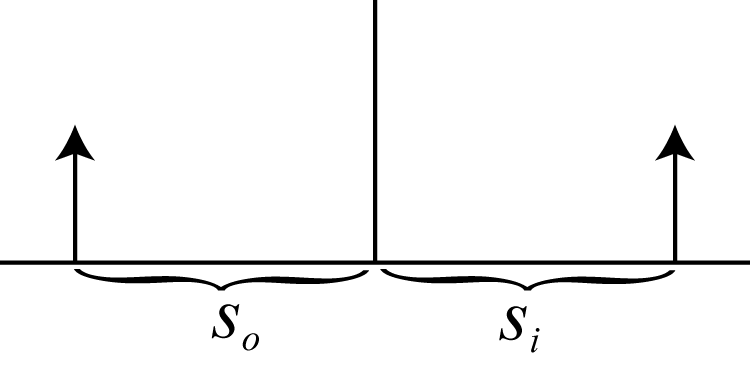
\includegraphics[scale=0.6]{images/PGRE_Figures_3p2p1_Flat_Mirror.png}
\end{center}
\(R=\infty\)
\begin{center}
  \begin{tabular}{ c | c  }
    Object Placement & Image \\ \hline%\cline{2-2}
    \multirow{3}{*}{ anywhere} & virtual \\
    & \(M=1\) \\
    & \(s_o=-s_i\) \\
    \hline
  \end{tabular}
\end{center}
Two \(\perp\) flat mirrors produce three virtual images (practice drawing the ray diagram).

\subsubsection{Concave Mirrors}
\begin{center}
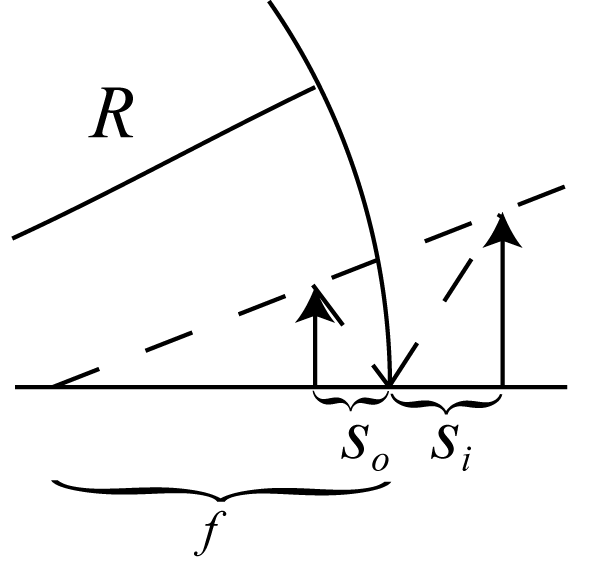
\includegraphics[scale=0.6]{images/PGRE_Figures_3p2p2_Concave_Mirror.png}
\end{center}
Using the convention of this document: \(R>0\)
\begin{center}
  \begin{tabular}{ c | c  }
    Object Placement & Image \\ \hline%\cline{2-2}
    \multirow{3}{*}{ \(s_o<f\)} & virtual \\
    & upright \\
    & \(M>1\) \\ \hline
    \(s_o=f\) & no image \\ \hline
    \multirow{2}{*}{ \(f<s_o<R\)} & real \\
    & \(M<-1\) \\ \hline
    \multirow{2}{*}{  \(s_o=R\)} & real \\
    & \(M=-1\) \\ \hline
     \multirow{2}{*}{  \(s_o>R\)} & real \\
    & \(-1<M<0\) \\
    \hline
  \end{tabular}
\end{center}

\subsubsection{Convex Mirrors}
\begin{center}
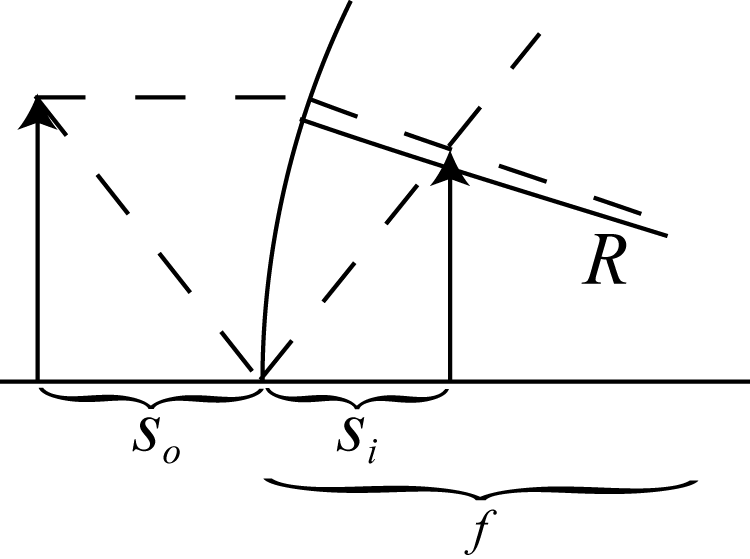
\includegraphics[scale=0.6]{images/PGRE_Figures_3p2p3_Convex_Mirror.png}
\end{center}
Using the convention of this document: \(R<0\)
\begin{center}
  \begin{tabular}{ c | c  }
    Object Placement & Image \\ \hline%\cline{2-2}
    \multirow{2}{*}{ anywhere} & virtual \\
    & \(0<M<1\) \\
    \hline
  \end{tabular}
\end{center}

\subsection{Refraction}
Index of Refraction: \(\displaystyle n=\frac{c}{v}\) where \(v\) is the speed of light in the material (\(n>1\) always)\\*
When light travels from one medium to another, the frequency and energy stay constant (but speed and wavelength change).\\*
Dispersion: \(n=n(\lambda)\) (the index of refraction depends on the wavelength of light)\\\\*
Images from Refraction: \(\displaystyle \frac{n_1}{s_o}+\frac{n_2}{s_i}=\frac{n_2-n_1}{R}\) (single surface)\\\\*
Thin Lens Equation: \(\displaystyle \frac{1}{f}=(n-1)\left(\frac{1}{R_1}-\frac{1}{R_2}\right)\)\\\\*
Lensmaker's Equation: \(\displaystyle \frac{1}{f}=(n-1)\left(\frac{1}{R_1}-\frac{1}{R_2}+\frac{(n-1)d}{nR_1R_2}\right)\)\\\\*
Sign convention: \(R\) and \(s_i\) are negative if measured from the same side as the object and are positive if measured from the opposite side as the object (opposite of mirrors).\\*
The \(d\) in the Lensmaker's equation is the thickness of the lens. For converging lenses it is the thickest width and for diverging lenses it is the smallest width.\\\\*
For a combination of lenses use the image of the first at the object of the second.\\*
For thin lenses in contact: \(\displaystyle\frac{1}{f}=\frac{1}{f_1}+\frac{1}{f_2}\)

\subsubsection{Snell's Law}
\(n_1\sin(\theta_1)=n_2\sin(\theta_2)\)\\\\*
Critical Angle: \(\displaystyle\theta_2=90^{\circ}\to \sin(\theta_c)=\frac{n_2}{n_1}\)

\subsubsection{Flat Refracting Surface}
\(\displaystyle R=\infty\to s_i=-\frac{n_2}{n_1}s_o\)

\subsubsection{Converging Lenses}
\(f>0\)\\*
A converging lens is thicker in the middle and thin at the ends.

\subsubsection{Diverging Lenses}
\(f<0\)\\*
A diverging lens is thinner in the middle and thick at the ends.

\subsection{Interference \& Diffraction}

\subsubsection{ Double-Slit Interference}
Sources must be coherent and monochromatic\\*
Screen must be far from the slits\\*
Bright Fringes: \(d\sin(\theta_{bright})=m\lambda\), \(m=0,\pm1,\pm2,\ldots\)\\*
Dark Fringes: \(d\sin(\theta_{dark})=\left(m+\frac{1}{2}\right)\lambda\)\\\\*
To get the position on the screen use \(\displaystyle\sin(\theta)\approx\frac{y}{L}\)

\subsubsection{Thin Films}
An electromagnetic wave undergoes a phase change of \(\pi\) upon reflection from a medium that has a higher index of refraction than the one in which the wave is traveling (wave on a string attached to a wall).\\\\*
This is for near normal incidence. In what follows \(m=0,1,2,\ldots\)\\*
Case: \(n_1<n_{film}<n_3\)\\*
Constructive Interference when: \(2n_{film}t=m\lambda\)\\*
Destructive Interference when: \(2n_{film}t=\left(m+\frac{1}{2}\right)\lambda\)\\*
Case: \(n_1<n_{film}>n_3\)\\*
Constructive Interference when: \(2n_{film}t=\left(m+\frac{1}{2}\right)\lambda\)\\*
Destructive Interference when: \(2n_{film}t=m\lambda\)\\*

\subsubsection{Single-Slit Diffraction}
Screen must be far from the slit\\*
Dark Fringes: \(a\sin(\theta_{dark})=m\lambda\), \(m=\pm1,\pm2,\pm3,\ldots\)

\subsubsection{Rayleigh Criterion}
This comes from the first order diffraction minimum.\\*
For Slit: \(\displaystyle\sin(\theta)=\frac{\lambda}{d}\)\\*
For Circular Aperture:  \(\displaystyle\sin(\theta)=1.22\frac{\lambda}{d}\)

\subsubsection{Diffraction (Interference) Grating}
Same as interference.\\*
Bright Fringes: \(d\sin(\theta_{bright})=m\lambda\), \(m=0,\pm1,\pm2,\ldots\)

\subsubsection{Bragg's Law}
This works for massive particles and photons (both have wave-like properties).\\*
Bright Fringes: \(2d\sin(\theta_{bright})=m\lambda\), \(m=1,2,3,\ldots\)

\subsection{Polarization}

\subsubsection{Polarizers}
If unpolarized light passes through a polarizer, the beam's intensity is halved.
If (plane) polarized light passes through a polarizer at a relative angle \(\phi-\theta\), the intensity is given by \(I_2=I_1\cos^2(\phi-\theta)\)

\subsubsection{Brewster's Law}
\begin{center}
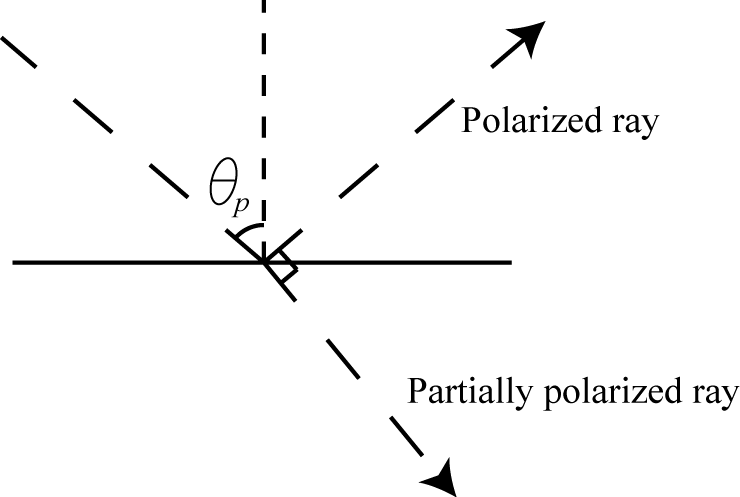
\includegraphics[scale=0.6]{images/PGRE_Figures_3p5p2_Brewsters_Law.png}
\end{center}
A reflected beam can be completely polarized if \(\tan(\theta_p)=n\)

\subsection{Rayleigh Scattering}
This type of scattering occurs when light elastically scatters off particles much smaller than the wavelength of the light.
Quantitatively, the intensity of the light that is scatter is related the wavelength of light by \(\displaystyle I\propto\frac{1}{\lambda^4}\).
This is the reason the sky looks blue and the sun appears yellow through Earth's atmosphere.
